\documentclass[a4paper]{article}
\usepackage[utf8]{inputenc}
\usepackage{amsmath}
\usepackage{amssymb}
\usepackage{siunitx}
\usepackage[ngerman]{babel}
\usepackage{pgfplots}
\usepackage{hyperref}
\usepackage{pgfplotstable}
\usepackage[section]{placeins}
\usepackage{enumitem}
\usepackage{float}
\usepackage{booktabs}
\usepackage[normalem]{ulem}
\usepackage{subcaption}
\usepackage{chngpage}
\usepackage[overload]{empheq}
\usepackage{todonotes}
\usepackage{graphicx}

\pgfplotsset{compat=1.15}

% Full Reference, produces: "Abbildung 3: Schaltplan"
\newcommand*{\fullref}[1]{\hyperref[{#1}]{\autoref*{#1}: \nameref*{#1}}}

\newcommand{\ugs}{U_{GS}}
\newcommand{\uds}{U_{DS}}
\newcommand{\uth}{U_{TH}}
\newcommand{\vo}{\si{V}}
\newcommand{\ma}{\si{mA}}

\newcommand{\trise}{t_\textit{Rise}}
\newcommand{\tfall}{t_\textit{Fall}}

\newcommand{\risetime}[2]{\trise=#1\si{#2}}
\newcommand{\falltime}[2]{\tfall=#1\si{#2}}



\newcommand{\stromverbrauchtable}[4]{
    \begin{tabular}{S|S|S}
        {$U_{IN}$} & {$U_{OUT}[V]$} & {$I_{ges}[mA]$}\\
        \hline
        {GND} & #1 & #2\\
        {$U_{DD}$} & #3 & #4
    \end{tabular}
}

\title{GPET\\ Auswertung Versuch 10\\ Gruppe 1}

\author{Jonas Otto\\ \href{mailto:jonas@jonasotto.com}{jonas@jonasotto.com} 
   \and Luca Krüger \\ \href{mailto:luca.krueger@uni-ulm.de}{luca.krueger@uni-ulm.de} }
\date{vom 19. Juni 2018}

\begin{document}

\maketitle

\newpage

\section{Vorbereitende Aufgaben und Fragen}
\subsection{Datenblätter}
\paragraph{BS270}
\begin{itemize}
    \item Eingangsspannung: $20\vo$
    \item Ausgangsspannung: $60\vo$
    \item Ausgangsstrom: $400\ma$
    \item Schwellspannung: $2.1\vo$
\end{itemize}

\paragraph{ZVP2106A}
\begin{itemize}
    \item Eingangsspannung: $20\vo$
    \item Ausgangsspannung: $\pm 60\vo$
    \item Ausgangsstrom: $280\ma$
    \item Schwellspannung:$-1.5\vo$ bis $-3.5\vo$
\end{itemize}

\subsection{Maximale Schaltfrequenz}
 In einer Periodendauer muss das von dem Mosfet erwartete Spannungslevel erreicht werden. Das ist abhängig von der Thresholdspannung und der Gate-Kapazität des Mosfets. Mit der ansteuernden Schaltung ergibt sich dann eine spezifische Rise-time $\trise$ und Fall-time $\tfall$.
 Die maximale Schaltfrequenz berechnet sich also durch $f_\text{max}=\frac{1}{2\cdot \max(\trise, \tfall)}$

\subsection{CMOS-NOR}
\begin{figure}[H]
    \centering
    \begin{subfigure}{.5\textwidth}
        \centering
        \begin{tabular}{c|c|c}
            $U_A$ & $U_B$ & $U_{OUT}$ \\ \hline
            0 & 0 & 1 \\
            0 & 1 & 0 \\
            1 & 0 & 0 \\
            1 & 1 & 0
        \end{tabular}
        \caption{Wahrheitstabelle}
        \label{tab:nor}
    \end{subfigure}%
    \begin{subfigure}{.5\textwidth}
        \centering
        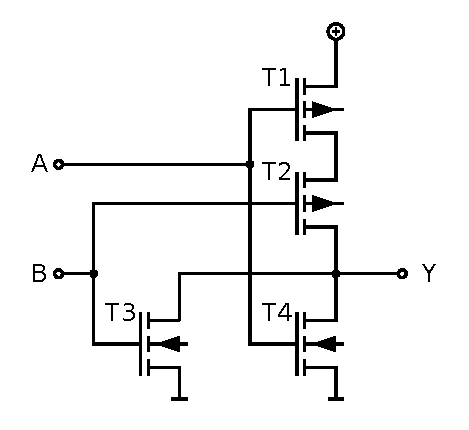
\includegraphics[width=.8\linewidth]{Vorbereitung/Cmos_nor.pdf}
        \caption{CMOS-NOR}
        \label{fig:nor-cmos}
    \end{subfigure}
    \caption{NOR}
    \label{fig:nor}
\end{figure}

\newpage

\section{Versuchsauswertung}
\subsection{Relais-Inverter}
\subsubsection{Stromverbrauch}
In diesem Versuch wird der Stromverbrauch des Relais gemessen. Dabei wurde dies mit konstanter Spannung $U_{DD}=10\si{V}$ geschaltet. Es ergibt sich ein Strom von $39\ma$.

\subsubsection{Dynamik des Relais}
In diesem Versuch wird die Inverterschaltung bei einer Frequenz von $10\si{Hz}$ betrieben.
Hier wurde zunächst die Reaktionszeit des Relais bestimmt.
Es dauert $7\si{ms}$, bis das Relais ausschaltet, und $16.8\si{ms}$ bis das Realis einschaltet. Dies resultiert in einer maximal nutzbaren Frequenz von $f=\frac{1}{2\cdot \max(\trise, \tfall)}=29.7\si{Hz}$. Wir stellen fest, dass bei dieser Frequenz das Relais nur sehr kurz im eingeschaltetem Zustand ist. Bei Frequenzen über $30\si{Hz}$ schaltet das Relais nicht mehr.

% \begin{figure}
%     \centering
%     \includegraphics{relais-schaltzeit}
%     \caption{Caption}
%     \label{fig:my_label}
% \end{figure}

\subsection{nMOS-Inverter}
\subsubsection{Stromverbrauch und Ausgangsspanne}
In diesem Versuch wird das Relais im Inverter durch einen nMOS Feldeffekttransistor ersetzt.
Beim Ändern der Eingangsspannung verhält sich die Schaltung wie in \autoref{tab:nmos-inverter-100} dargestellt.
Im weiteren Verlauf wird der Widerstand $R$ von $100\si{\ohm}$ auf $1\si{k\ohm}$ erhöht. Das Verhalten der Schaltung entspricht nun \autoref{tab:nmos-inverter-1k}.

\begin{figure}[H]
    \centering
    \begin{subfigure}{0.5\textwidth}
        \centering
        \stromverbrauchtable{5}{0.005}{0.2}{49}
        \caption{$R=100\si{\ohm}$}
        \label{tab:nmos-inverter-100}
    \end{subfigure}%
    \begin{subfigure}{0.5\textwidth}
        \centering
        \stromverbrauchtable{5}{0.005}{0.2}{5}
        \caption{$R=1\si{k\ohm}$}
        \label{tab:nmos-inverter-1k}
    \end{subfigure}
    \caption{Stromverbrauch und Ausgangsspanne des nMOS-Inverters}
    \label{fig:nmos-inverter}
\end{figure}

\subsubsection{Dynamik}
Der Inverter wird nun mit einer Rechteckspannung mit $1\si{MHz}$ gesteuert.
Die gemessene Anstiegszeit der Schaltung beträgt $\trise=\si{\micro s}$, die Abfallzeit $\tfall=\si{\micro s}$.
Die theoretische maximale Frequenz beträgt $f=\frac{1}{t}=\frac{1}{2\cdot \max(\trise, \tfall)}=\si{Hz}$.
Wenn der Pull-Up Widerstand auf $1\si{k\ohm}$ erhöht wird, beträgt $\trise=\si{\micro s}$, $\tfall=\si{\micro s}$, und damit $f=\frac{1}{t}=\frac{1}{2\cdot \max(\trise, \tfall)}=\si{Hz}$.

\begin{table}[H]
    \centering
    \begin{tabular}{S|S|S|S}
        {$R$} & {$\trise[ns]$} & {$\tfall[ns]$} & {$f_{max}[MHz]$}\\
        \hline
        \num{100}\si{\ohm} & 15 & 8.4 & 33.3 \\
        \num{1}\si{k\ohm} & 324 & 8.4 & 1.5
    \end{tabular}
    \caption{Timing NMOS Inverter}
    \label{tab:nmos-inverter-timing}
\end{table}

% \begin{figure}[H]
%     \centering
%     \includegraphics[width=0.8\textwidth]{nmos-inverter-risetime-100.png}
%     \caption{Messung von $t_{rise}$ mit $R=100\si{\ohm}$ beim NMOS Inverter}
%     \label{fig:nmos-inverter-risetime-100}
% \end{figure}

% \begin{figure}[H]
%     \centering
%     \includegraphics[width=0.8\textwidth]{nmos-inverter-falltime-100.png}
%     \caption{Messung von $t_{fall}$ mit $R=100\si{\ohm}$ beim NMOS Inverter}
%     \label{fig:nmos-inverter-falltime-100}
% \end{figure}

%für verschiedene widerstände 100,1k wie in anleitung

\subsection{CMOS-Inverter}
In diesem Versuch wird der Inverter des letzten Versuchs dahingehend verändert, dass der Pullup Widerstand durch einen p-Kanal Mosfet ersetzt wird.
\subsubsection{Stromerbrauch und Ausgangsspanne}
Der Stromverbrauch ist, der die Ausgangsspanne, wie in \autoref{tab:cmos-inverter} ersichtlich ist.

\begin{table}[H]
    \centering
    \stromverbrauchtable{5}{0.005}{0}{0}
    \caption{Stromerbrauch und Ausgangsspanne des CMOS-Inverters}
    \label{tab:cmos-inverter}
\end{table}

\subsubsection{Dynamik}

Hier wird der Inverter wieder benutzt, um ein Rechtecksignal mit $f=1\si{MHz}$ zu invertieren.
Eine Messung der Risetime und Falltime ergibt $\risetime{26.4}{ns}$ und $\falltime{10.6}{ns}$.
Die theoretische Maximalfrequenz beträgt $f=\frac{1}{2\cdot \max(\trise , \tfall)}=18.9\si{MHz}$.

% \begin{figure}[H]
%     \centering
%     \includegraphics[width=0.8\textwidth]{cmos-inverter-risetime-100.png}
%     \caption{Messung von $t_{rise}$ mit $R=100\si{\ohm}$ beim CMOS Inverter}
%     \label{fig:cmos-inverter-risetime}
% \end{figure}

% \begin{figure}[H]
%     \centering
%     \includegraphics[width=0.8\textwidth]{cos-inverter-falltime-100.png}
%     \caption{Messung von $t_{fall}$ mit $R=100\si{\ohm}$ beim CMOS Inverter}
%     \label{fig:cmos-inverter-falltime}
% \end{figure}

% Zum Inverter lässt sich abschließend sagen, dass die CMOS Variante vorzuziehen ist, wenn hohen Frequenzen und kleine Ströme verwendet werden. Ist hingegen ein nicht hochfrequentes Signal zu invertieren, und sind die Ansprüche an den Ausgangsstrom höher, ist ein Relais im Vorteil. 

\subsection{CMOS NOR}
In diesem Versuch wurde ein CMOS NOR Gate nach \autoref{fig:nor-cmos} aufgebaut.
\end{document}
